\chapter{Computing Solutions to Non-linear Equations}

So far, we are computing solutions using direct methods -- we follow an algorithm, and after a fixed number of steps, we obtain a solution. However, to solve for non-linear equations, we need to apply an indirect, iterative method.

\section{Roots of a Function}

Determine the roots of a general equation of the form \( f(x) = 0 \). That is, find \( x^\ast \) such that \( f(x^\ast) = 0 \).

\begin{note}
    We stick with \( f: \R \to \R \).
\end{note}

How to know when a root must exist? We use the Intermediate Value Theorem (IVT).

\begin{theorem}[Intermediate Value Theorem]
    For a continuous function \( f \in C[a, b] \), if \( v \) is any number between \( f(a) \) and \( f(b) \), then there exists a number \( c \in [a, b] \) such that \( f(c) = v \).
\end{theorem}

\begin{remark}
    \( c \) has to exist, but does \textbf{not} have to be unique.
\end{remark}

We could apply IVT to obtain the following algorithm:
\begin{itemize}
    \item \( x = L \), \( x = R \), \( L < R \)
    \item \( f(L) \) and \( f(R) \) have opposite signs, i.e. \( f(L) \cdot f(R) < 0 \)
    \item By IVT, there has to be a root \( x^\ast \) in the interval \( [L, R] \) with \( f(x^\ast) = 0 \)
\end{itemize}

\begin{example}
    Consider \[
        f(x) = \cos(x) - x \qquad x \in [0, \pi/2]
    \]

    \begin{figure}[H]
        \centering
        \begin{tikzpicture}
            \draw[->] (-1, 0) -- (2, 0) node[right] {\( x \)};
            \draw[->] (0, -2) -- (0, 1.2) node[above] {\( f(x) \)};

            \draw[domain=0:pi/2, smooth, variable=\x, blue] plot (\x, {cos(\x r) - \x});

            \draw[red] (pi/8, 0) -- (pi/8, {cos(pi/8 r) - pi/8}) node[black,above] {\( \frac{\pi}{8} \)};
            \draw[red] (pi/4, {cos(pi/4 r) - pi/4}) -- (pi/4, 0) node[black,below] {\( \frac{\pi}{4} \)};
        \end{tikzpicture}
    \end{figure}

    We have
    \begin{itemize}
        \item \( f(0) = 1 \), \( f(\pi/2) = -\pi/2 \)
        \item \( f(x) \) is continuous
    \end{itemize}

    By IVT, there exists a root \( x^\ast \) in the interval \( [0, \pi/2] \) such that \( f(x^\ast) = 0 \).

        {~~~}

    \begin{enumerate}
        \item Consider the midpoint of \( [0, \pi/2] \), \[
                  m_1 = L + \frac{1}{2}(R - L) = \frac{\pi}{4}
              \] and we approximate \( x^\ast \) by \( m_1 = \frac{\pi}{4} \). Our error is bounded by \[
                  e_1 = | m_1 - x^\ast | \leq \frac{1}{2} | R - L | = \frac{\pi}{4} \doteq 0.785
              \]
              If we evaluate \( f(\pi / 4) \), we get \[
                  f(\pi / 4) = \cos(\pi / 4) - \frac{\pi}{4} = \frac{\sqrt{2}}{2} - \frac{\pi}{4} \doteq 0.07829
              \] which is not close to 0. We need to refine our estimate.

        \item We observe that if we shrink the interval, we can get a better estimate.

              By IVT, there must be a root between \( [0, \pi/4] \). We have \[
                  m_2 = \frac{\pi}{8}
              \] and the error is bounded by \[
                  e_2 = | m_2 - x^\ast | \leq \frac{1}{2} | R - L | = \frac{\pi}{8} \doteq 0.393
              \]
              Evaluating \( f(\pi / 8) \), we get \[
                  f(\pi / 8) = \cos(\pi / 8) - \frac{\pi}{8} \doteq 0.5312
              \] and by IVT, there must be a root between \( [\pi/8, \pi/4] \).
    \end{enumerate}

    \begin{table}[H]
        \centering
        \begin{tabular}{c|c|c|c|c|c|c}
            Iteration & \( L_i \)    & \( R_i \)    & \( m_i \)
                      & \( f(L_i) \) & \( f(R_i) \) & \( f(m_i) \) \\ \hline
            \(1\)     & \(0\)        & \(\pi/2\)    & \(\pi/4\)
                      & \(+\)        & \(+\)        & \( -0.078 \) \\
            \(2\)     & \(0\)        & \(\pi/4\)    & \(\pi/8\)
                      & \(+\)        & \(-\)        & \( +0.531 \) \\
            \(3\)     & \(\pi/8\)    & \(\pi/4\)    & \(3\pi/16\)
                      & \(+\)        & \(-\)        & \( +0.242 \) \\
            \(4\)     & \(\pi/8\)    & \(3\pi/16\)  & \(5\pi/32\)
                      & \(+\)        & \(-\)        & \( +0.086 \) \\
            etc.
        \end{tabular}
        \caption{Iteration table for the \( [L_i, R_i] \) intervals}
    \end{table}
    Our error in approximating \( x^\ast \) by \( m_i \) is given by \[
        e_i \leq \frac{1}{2} | R_i - L_i |
    \]
    When do we terminate the algorithm?

    \begin{enumerate}
        \item we can stop when the bound on the error is sufficiently small, \[
                  \frac{1}{2} | R_i - L_i | \leq \text{ABS\_TOL}
              \] We take the approximation of the root as \[
                  x^\ast = L_i + \frac{1}{2} (R_i - L_i)
              \]
        \item We could also stop when a maximum number of iterations is reached.
        \item We could also defined a relative tolerance instead of an absolute tolerance, \[
                  \frac{1}{2} | R_i - L_i | \leq \text{REL\_TOL} \cdot | x^\ast |
              \]
        \item We could also stop when \( f(m) \) is small enough

              Note that we could be tricked, as we could have \( f(a) \), but \( | a - x^\ast | \) not necessarily small.
    \end{enumerate}

    In practice, we often combine \( 1 \) and \( 4 \).
\end{example}

\section{Bisection Method}

Suppose we are given a continuous function \( f(x) \) and \( L, R \) such that \( L < R \), \[
    f(L) \cdot f(R) < 0
\]

\begin{algorithm}[H]
    \begin{algorithmic}[1]
        \While {\( \frac{1}{2} | R - L | > \text{ABS\_TOL} \)}
        \State \( M \gets (R + L) / 2 \)
        \If {\Call{Sign}{\(f(L)\)} == \Call{Sign}{\(f(m)\)}}
        \State \( L \gets M \)
        \Else
        \State \( R \gets M \)
        \EndIf
        \EndWhile
        \State \( x^\ast \gets L + (R - L) / 2 \)
        \State \Return \( x^\ast \)
    \end{algorithmic}
\end{algorithm}

We have errors \begin{align*}
    e_1 & = | m_1 - x^\ast | \leq \frac{1}{2} ( R_1 - L_1 )
    \\
    e_2 & = | m_2 - x^\ast | \leq \frac{1}{2} ( R_2 - L_2 )
    = \frac{1}{4} ( R_1 - L_1 )
    \\
        & \vdots
    \\
    e_n & = | m_n - x^\ast | \leq \frac{1}{2^n} ( R_1 - L_1 )
\end{align*}

\begin{itemize}
    \item \textbf{Pros}
          \begin{itemize}
              \item Easy to implement
              \item Given interval bracket of root, guaranteed to converge (not often true for other methods)
              \item Only require knowledge of \( f(x) \), and not derivatives.
          \end{itemize}

    \item \textbf{Cons}
          \begin{itemize}
              \item Finding an interval bracket can be hard
              \item Convergence is slow, and convergence behaviour is not uniform
              \item Does not make use of much information about \( f(x) \)
          \end{itemize}
\end{itemize}

\begin{example}
    Suppose we want to find the root of \[
        f(x) = x - 0.2 \sin(x) - 0.5
    \] with absolute error \( | x_i - x^\ast | \leq 5 \times 10^{-7} \).

    How many iterations is required to achieve this error?

    {~~~}

    Recall that we are given \[
        e_n \leq \frac{1}{2^n} ( R_1 - L_1 )
    \] and thus \[
        e_n \leq \frac{1}{2^n} (1 - 0) \leq 5 \times 10^{-7}
    \] We solve for \( n \) to get \begin{align*}
        2^n
         & \geq 0.2 \times 10^7
        \\
        n
         & \geq \log_2 \left( 0.2 \times 10^7 \right) \doteq 20.93
    \end{align*}
    Thus, we need at least 21 iterations.

        {~~~}

    Indeed, we verify with python:

    \begin{longtable}[t]{c|c|c|c|c|c|c|c}
        Step                  &
        \( L \)               & \( f(L) \)             &
        \( R \)               & \( f(R) \)             &
        \( M \)               & \( f(M) \)             & Max Error        \\ \hline \hline
        1                     &
        \texttt{0.000000E+00} & \(-\)                  &
        \texttt{1.000000E+00} & \(+\)                  &
        \texttt{5.000000E-01} & \texttt{-9.58511E-02}  & \texttt{5.0-01 } \\
        2                     &
        \texttt{5.000000E-01} & \(-\)                  &
        \texttt{1.000000E+00} & \(+\)                  &
        \texttt{7.500000E-01} & \texttt{1.136722E-01}  & \texttt{2.5E-01} \\
        3                     &
        \texttt{5.000000E-01} & \(-\)                  &
        \texttt{7.500000E-01} & \(+\)                  &
        \texttt{6.250000E-01} & \texttt{7.980545E-03}  & \texttt{1.2E-01} \\
        4                     &
        \texttt{5.000000E-01} & \(-\)                  &
        \texttt{6.250000E-01} & \(+\)                  &
        \texttt{5.625000E-01} & \texttt{-4.416053E-02} & \texttt{6.2E-02} \\
        5                     &
        \texttt{5.625000E-01} & \(-\)                  &
        \texttt{6.250000E-01} & \(+\)                  &
        \texttt{5.937500E-01} & \texttt{-1.814463E-02} & \texttt{3.1E-02} \\
        6                     &
        \texttt{5.937500E-01} & \(-\)                  &
        \texttt{6.250000E-01} & \(+\)                  &
        \texttt{6.093750E-01} & \texttt{-5.096014E-03} & \texttt{1.6E-02} \\
        7                     &
        \texttt{6.093750E-01} & \(-\)                  &
        \texttt{6.250000E-01} & \(+\)                  &
        \texttt{6.171875E-01} & \texttt{1.438734E-03}  & \texttt{7.8E-03} \\
        8                     &
        \texttt{6.093750E-01} & \(-\)                  &
        \texttt{6.171875E-01} & \(+\)                  &
        \texttt{6.132812E-01} & \texttt{-1.829518E-03} & \texttt{3.9E-03} \\
        9                     &
        \texttt{6.132812E-01} & \(-\)                  &
        \texttt{6.171875E-01} & \(+\)                  &
        \texttt{6.152344E-01} & \texttt{-1.956125E-04} & \texttt{2.0E-03} \\
        10                    &
        \texttt{6.152344E-01} & \(-\)                  &
        \texttt{6.171875E-01} & \(+\)                  &
        \texttt{6.162109E-01} & \texttt{6.215054E-04}  & \texttt{9.8E-04} \\
        11                    &
        \texttt{6.152344E-01} & \(-\)                  &
        \texttt{6.162109E-01} & \(+\)                  &
        \texttt{6.157227E-01} & \texttt{2.129326E-04}  & \texttt{4.9E-04} \\
        12                    &
        \texttt{6.152344E-01} & \(-\)                  &
        \texttt{6.157227E-01} & \(+\)                  &
        \texttt{6.154785E-01} & \texttt{8.656611E-06}  & \texttt{2.4E-04} \\
        13                    &
        \texttt{6.152344E-01} & \(-\)                  &
        \texttt{6.154785E-01} & \(+\)                  &
        \texttt{6.153564E-01} & \texttt{-9.347883E-05} & \texttt{1.2E-04} \\
        14                    &
        \texttt{6.153564E-01} & \(-\)                  &
        \texttt{6.154785E-01} & \(+\)                  &
        \texttt{6.154175E-01} & \texttt{-4.241132E-05} & \texttt{6.1E-05} \\
        15                    &
        \texttt{6.154175E-01} & \(-\)                  &
        \texttt{6.154785E-01} & \(+\)                  &
        \texttt{6.154480E-01} & \texttt{-1.687741E-05} & \texttt{3.1E-05} \\
        16                    &
        \texttt{6.154480E-01} & \(-\)                  &
        \texttt{6.154785E-01} & \(+\)                  &
        \texttt{6.154633E-01} & \texttt{-4.110413E-06} & \texttt{1.5E-05} \\
        17                    &
        \texttt{6.154633E-01} & \(-\)                  &
        \texttt{6.154785E-01} & \(+\)                  &
        \texttt{6.154709E-01} & \texttt{2.273095E-06}  & \texttt{7.6E-06} \\
        18                    &
        \texttt{6.154633E-01} & \(-\)                  &
        \texttt{6.154709E-01} & \(+\)                  &
        \texttt{6.154671E-01} & \texttt{-9.186596E-07} & \texttt{3.8E-06} \\
        19                    &
        \texttt{6.154671E-01} & \(-\)                  &
        \texttt{6.154709E-01} & \(+\)                  &
        \texttt{6.154690E-01} & \texttt{6.772177E-07}  & \texttt{1.9E-06} \\
        20                    &
        \texttt{6.154671E-01} & \(-\)                  &
        \texttt{6.154690E-01} & \(+\)                  &
        \texttt{6.154680E-01} & \texttt{-1.207210E-07} & \texttt{9.5E-07} \\
        21                    &
        \texttt{6.154680E-01} & \(-\)                  &
        \texttt{6.154690E-01} & \(+\)                  &
        \texttt{6.154685E-01} & \texttt{2.782483E-07}  & \texttt{4.8E-07}
        \\
        \caption{Bisection method for \( f(x) = x - 0.2 \sin(x) - 0.5 \)}
    \end{longtable}
\end{example}

\newpage
\section{Fixed Point Iteration}

\begin{note}
    The problem of finding \( x^\ast \) such that \( f(x^\ast) = 0 \) is equivalent to the problem of finding \( x = p^\ast \) such that \( g(p^\ast) = p^\ast \) where \( g(x) = x - f(x) \).
\end{note}

\begin{definition}[Fixed Point]\index{Fixed Point}
    A point \( p^\ast \) is called a \term{fixed point} of a function \( g(x) \) if and only if \( g(p^\ast) = p^\ast \).
\end{definition}

\begin{example}
    Consider \( g(x) = x^3 - x - 1 \).
    \begin{figure}[H]
        \centering
        \begin{tikzpicture}
            \begin{axis}[
                    axis lines = middle,
                    xlabel = \( x \),
                    ylabel = \( g(x) \),
                    xmin = -2, xmax = 2,
                    ymin = -2, ymax = 2,
                ]
                \addplot[domain=-2:2, samples=100, color=blue]{x^3 - x - 1};
                \addplot[domain=-2:2, samples=100, color=red]{x};

                \addplot[only marks, mark=*, color=red] coordinates {(-1, -1) (-0.618, -0.618) (1.618, 1.618)};
            \end{axis}
        \end{tikzpicture}
        \caption{Graph of \( g(x) = x^3 - x - 1 \). The fixed points of \( g \) are the points on \( g \) intersecting the line \( y = x \): \( x = -1, \sfrac{1}{2}(1 \pm \sqrt5) \)}
    \end{figure}
\end{example}

We could use \term{fixed point iteration} (or, \term{functional iteration}) to find the fixed point of a function.\index{Fixed Point Iteration}\index{Functional Iteration}

\subsection{Fixed Point Iteration}

Define the sequence \[
    x_0 \text{ given } \qquad x_{i+1} = g(x_i)
\] for \( i = 0, 1, 2, \dots \). If it converges, then \[
    \lim_{i \to \infty} x_i = x^\ast
\]

\begin{note}
    Unlike bisection method, we do not have a guarantee of convergence.
\end{note}

\begin{example}
    Find a root of \[
        f(x) = x - 0.2 \sin (x) - 0.5
    \]

    Via the bisection method, we get a root at \( x^\ast \doteq 0.6514685 \) in 21 iterations.

        {~~~}

    We now use the fixed point iteration method to find the root. Define \[
        g(x) = 0.2 \sin(x) + 0.5 \qquad f(x) = x - g(x)
    \] and we apply functional iteration to this \( g(x) \) with \( x_0 = 0 \). Compute \[
        x_0 = 0 \qquad x_{i+1} = g(x_i)
    \] until \[
        | x_{i+1} - x_i | \leq 5 \times 10^{-7}
    \]

    \begin{table}[H]
        \centering
        \begin{tabular}{c|c|c}
            \( i \) & \( x_i \)             & \( | x_i - x_{i-1} | \)
            \\ \hline \hline
            0       & \texttt{0.000000E+00} &                         \\
            1       & \texttt{5.000000E-01} & \texttt{5.0e-01}        \\
            2       & \texttt{5.958851E-01} & \texttt{9.6E-02}        \\
            3       & \text{6.122483e-01}   & \texttt{1.6E-02}        \\
            4       & \text{6.149418e-01}   & \texttt{2.7E-03}        \\
            5       & \text{6.153822e-01}   & \texttt{4.4E-04}        \\
            6       & \text{6.154541e-01}   & \texttt{7.2E-05}        \\
            7       & \text{6.154659e-01}   & \texttt{1.2E-05}        \\
            8       & \text{6.154678e-01}   & \texttt{1.9E-06}        \\
            9       & \text{6.154681e-01}   & \texttt{3.1E-07}
        \end{tabular}
    \end{table}
\end{example}

\begin{remark}
    The value of \( x_0 \) may affect the number of iterations required to converge.

    \begin{table}[H]
        \centering
        \begin{tabular}{c|c}
            \( x_0 \)   & Steps to Convergence
            \\ \hline
            \( 1 \)     & 9
            \\
            \( -1 \)    & 10
            \\
            \( 10 \)    & 10
            \\
            \( -100 \)  & 7
            \\
            \( 1000 \)  & 9
            \\
            \( -1000 \) & 10
        \end{tabular}
    \end{table}
\end{remark}

% TODO: Plot

\begin{example}
    Use fixed point iteration to find the root of \[
        f(x) = x^3 - x - 1
    \]
    We note that \[
        f(x) = (x^3 - 1) - x
    \] Define \[
        g(x) = x^3 - 1
    \] and we try fixed iteration on \( g(x) \) from \( x_0 = 1 \).

    \begin{table}[H]
        \centering
        \begin{tabular}{c|c|c}
            \( i \) & \( x_i \)               & \( | x_i - x_{i-1} | \)
            \\ \hline \hline
            0       & \texttt{1.000000e+00}   &
            \\
            1       & \texttt{0.000000e+00}   & \texttt{1.0e+00}
            \\
            2       & \texttt{-1.000000e+00}  & \texttt{1.0e+00}
            \\
            3       & \texttt{-2.000000e+00}  & \texttt{1.0e+00}
            \\
            4       & \texttt{-9.000000e+00}  & \texttt{7.0e+00}
            \\
            5       & \texttt{-7.300000e+02}  & \texttt{7.2e+02}
            \\
            6       & \texttt{-3.890170e+08}  & \texttt{3.9e+08}
            \\
            7       & \texttt{-5.887159e+25}  & \texttt{5.9e+25}
            \\
            8       & \texttt{-2.040409e+77}  & \texttt{2.0e+77}
            \\
            9       & \texttt{-8.494771e+231} & \texttt{8.5e+231}
        \end{tabular}
    \end{table}
    This series diverges, and we do not get a root. We try another starting point, \( x_0 = 2 \).
    \begin{table}[H]
        \centering
        \begin{tabular}{c|c|c}
            \( i \) & \( x_i \)              & \( | x_i - x_{i-1} | \)
            \\ \hline \hline
            0       & \texttt{2.000000e+00}  &
            \\
            1       & \texttt{7.000000e+00}  & \texttt{5.0e+00}
            \\
            2       & \texttt{3.420000e+02}  & \texttt{3.4e+02}
            \\
            3       & \texttt{4.000169e+07}  & \texttt{4.0e+07}
            \\
            4       & \texttt{6.400810e+22}  & \texttt{6.4e+22}
            \\
            5       & \texttt{2.622435e+68}  & \texttt{2.6e+68}
            \\
            6       & \texttt{1.803492e+205} & \texttt{1.8e+205}
        \end{tabular}
    \end{table}

    Alternatively, we observe that \[
        f(x) = x^3 - (x + 1)
    \] and try \[
        g(x) = (x + 1)^{\sfrac{1}{3}}
    \] with \( x_0 = 1 \).

    \begin{table}[H]
        \centering
        \begin{tabular}{c|c|c}
            \( i \) & \( x_i \)             & \( | x_i - x_{i-1} | \)
            \\ \hline \hline
            0       & \texttt{1.000000e+00} &
            \\
            1       & \texttt{1.259921e+00} & \texttt{2.6e-01}
            \\
            2       & \texttt{1.312294e+00} & \texttt{5.2e-02}
            \\
            3       & \texttt{1.322354e+00} & \texttt{1.0e-02}
            \\
            4       & \texttt{1.324269e+00} & \texttt{1.9e-03}
            \\
            5       & \texttt{1.324633e+00} & \texttt{3.6e-04}
            \\
            6       & \texttt{1.324702e+00} & \texttt{6.9e-05}
            \\
            7       & \texttt{1.324715e+00} & \texttt{1.3e-05}
            \\
            8       & \texttt{1.324717e+00} & \texttt{2.5e-06}
            \\
            9       & \texttt{1.324718e+00} & \texttt{4.7e-07}
        \end{tabular}
    \end{table}
    which converges to \( x^\ast \doteq 1.324718 \) in 9 iterations.
\end{example}

\subsection{Convergence of Fixed Point Iteration}

\begin{theorem}[Fixed Point Theorem]
    \bold{(a)} If \( g \in C[a, b] \) with \( a < b \), and if for all \( x \in [a, b] \), \( g(x) \in [a, b] \), then \( g \) must have a fixed point in the interval \( [a, b] \).

        {~~~}

    \bold{(b)} Furthermore, if \( g'(x) \) exists on \( (a, b) \) and \( | g'(x) | \leq k < 1 \) for some constant \( k \) and all \( x \in (a, b) \), then the fixed point in \( [a, b] \) is unique.
\end{theorem}

\begin{proof}(Part (a) Existence)

    If \( g(a) = a \), or \( g(b) = b \), then \( g(x) \) has a fixed point in \( [a, b] \), namely \( a \) or \( b \).

    Otherwise, \( g(a) \neq a \) and \( g(b) \neq b \).

    Then, \( g(a) > a \) and \( g(b) < b \).

    Since \( g(x) \in [a, b] \) for all \( x \in [a, b] \), we have \[
        g(a) - a > 0 \qquad g(b) - b < 0
    \]
    Take \( h(x) = g(x) - x \). Then,
    \begin{enumerate}
        \item \( h(x) \) is continuous in \( [a, b] \)
        \item \( h(a) > 0 \)
        \item \( h(b) < 0 \)
    \end{enumerate}
    and hence by IVT, \( h(x) \) has a root between \( a, b \).

    That is, exists \( x^\ast in [a, b] \) such that \[
        h(x^\ast) = 0 \implies g(x^\ast) - x^\ast = 0 \implies g(x^\ast) = x^\ast
    \] and \( x^\ast \in [a, b] \) is a fixed point of \( g(x) \).
\end{proof}

\begin{proof}(Part (b) Uniqueness)

    Suppose for contradiction that \( p, q \) are two fixed points of \( g(x) \) in \( [a, b] \) with \( p \neq q \).

    Then, by the mean value theorem, exists \( c \in (p, q) \) such that \[
        g'(c) = \frac{g(q) - g(p)}{q - p}
    \]
    Then we have \begin{align*}
        | p - q | & = | g(p) - g(q) |                       \\
                  & = | g'(c) | \cdot | p - q |             \\
                  & \leq k | p - q |                        \\
                  & < | p - q | \text{ (since \( k < 1 \))}
    \end{align*}
    We have a contradiction that \( | p - q | < | p - q | \).

    Thus, \( p, q \) must be equal, and the fixed point of \( g(x) \) is unique in \( [a, b] \).
\end{proof}

\begin{example}
    Consider \[
        g(x) = 0.2 \sin(x) + 0.5
    \] between the interval \( [0, 1] \).

    \begin{figure}[H]
        \centering
        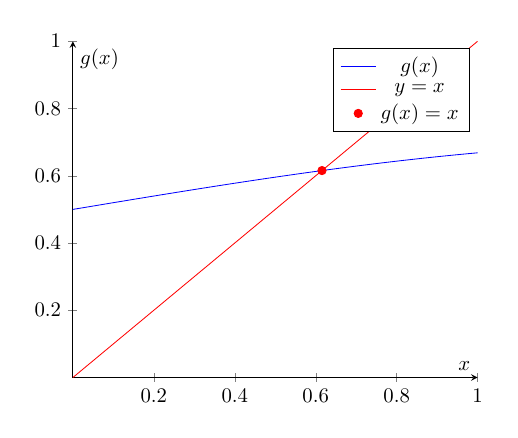
\begin{tikzpicture}[scale=0.75]
            \begin{axis}[
                    axis lines = middle,
                    xlabel = \( x \),
                    ylabel = \( g(x) \),
                    xmin = 0, xmax = 1,
                    ymin = 0, ymax = 1,
                ]
                \addplot[domain=-0.5:1.5, samples=100, color=blue]{0.2 * sin(deg(x)) + 0.5};
                \addplot[domain=-0.5:1.5, samples=100, color=red]{x};
                \addplot[only marks, mark=*, color=red] coordinates {(0.61547, 0.61547)};

                \addlegendentry{\( g(x) \)}
                \addlegendentry{\( y = x \)}
                \addlegendentry{\( g(x) = x \)}

            \end{axis}
        \end{tikzpicture}
        % \caption{Graph of \( g(x) = 0.2 \sin(x) + 0.5 \) in the interval \( [0, 1] \). The fixed point of \( g \) is the point on \( g \) intersecting the line \( y = x \): \( x = 0.61547 \)}
    \end{figure}

    \begin{itemize}
        \item Since \( \sin(x) \in [-1, 1] \) for all \( x \), we have \[
                  g(x) \in [0.2 \cdot (-1) + 0.5, 0.2 \cdot 1 + 0.5] = [0.3, 0.7] \subsetneq [0, 1]
              \]

              \( g(x) \) is continuous in \( [0, 1] \), and thus by the fixed point theorem, \( g(x) \) has a fixed point in \( [0, 1] \).

        \item We have \[
                  g'(x) = 0.2 \cos(x)
              \] and since \( \cos(x) \in [0, 1] \), we have \[
                  | g'(x) | \leq 0.2 < 1
              \] for all \( x \in [0, 1] \).

              Thus, by the fixed point theorem, \( g(x) \) has a unique fixed point in \( [0, 1] \).
    \end{itemize}
\end{example}

\begin{remark}
    The conditions of the theorem are sufficient, but not necessary.
\end{remark}

When will functional iteration converge? Recall that for functional iteration, we are given \( x_0 \) and compute the series \( x_{i+1} = g(x_i) \) for \( i = 0, 1, 2, \dots \) until \( | x_{i+1} - x_i | \leq \text{ABS\_TOL} \).

    {~~~}

Depending on the derivative at the root, \( g'(x^\ast) \), we can have different convergence behaviour.

Suppose \[
    g(x^\ast) = x^\ast
\] and that the fixed point iteration gives \[
    x_i = x^\ast + h
\] where \( h \) is small.

Then, \begin{align*}
    x_{i+1} & = g(x_i)                                                        \\
            & = g(x^\ast + h)                                                 \\
            & = g(x^\ast) + h g'(x^\ast) + \frac{h^2}{2!} g''(x^\ast) + \dots \\
            & \doteq g(x^\ast) + h g'(x^\ast)
\end{align*} so \begin{align*}
    x_{i+1} - g(x^\ast) & \doteq h g'(x^\ast) \\
    x_{i+1} - x^\ast    & \doteq h g'(x^\ast)
\end{align*}
Thus, error in \( (i+1)^th \) approximation is \[
    | x_{i+1} - x^\ast | = | g'(x^\ast) | \cdot | x_i - x^\ast |
\] which is \[
    | g'(x^\ast) | \times \text{the error in the \( i^{th} \) approximation}
\] and the convergence behaviour depends on the value of \( g'(x^\ast) \).

\begin{itemize}
    \item If \( |g'(x^\ast)| < 1 \), then \( x_{i+1} \) is closer to \( x^\ast \) than \( x_i \), and the error converges linearly. This is called \term{attracting fixed point}.
    \item If \( |g'(x^\ast)| = 1 \), then \( x_{i+1} \) is farther from \( x^\ast \) than \( x_i \), and the error diverges. This is called \term{repulsing fixed point}.
\end{itemize}

\begin{example}
    Consider the functions
    \[
        g_1(x) = \frac{1}{2} \left( x^3 + x \right)
        \qquad \text{and} \qquad
        g_2(x) = -\frac{1}{2} \left( x^3 + 1 \right)
    \]
    Differentiating \( g_1, g_2 \) we get \[
        {g_1}'(x) = \frac{1}{2} (3x^2 + 1)
        \qquad \text{and} \qquad
        {g_2}'(x) = -\frac{1}{2} (3x^2 + 1)
    \]

    \begin{itemize}
        \item \( g_1 \) has three fixed points \[
                  x = -1 \qquad x = 0 \qquad x = 1
              \] and first derivatives \[
                  g'(-1) = 2 \qquad g'(0) = \frac{1}{2} \qquad g'(1) = 2
              \]
    \end{itemize}

    \begin{figure}[H]
        \centering
        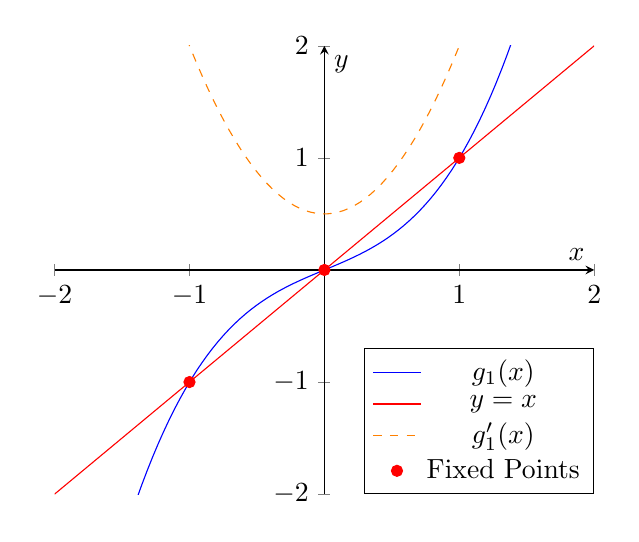
\begin{tikzpicture}
            \begin{axis}[
                    axis lines = middle,
                    xlabel = \( x \),
                    ylabel = \( y \),
                    xmin = -2, xmax = 2,
                    ymin = -2, ymax = 2,
                    legend style = {at={(1, 0)}, anchor = south east},
                ]
                \addplot[domain=-2:2, samples=100, color=blue]{(x^3 + x) / 2};
                \addplot[domain=-2:2, samples=100, color=red]{x};
                \addplot[domain=-2:2, samples=100, color=orange, dashed]{(3 * x^2 + 1) / 2};

                \addplot[only marks, mark=*, color=red] coordinates {(-1, -1) (0, 0) (1, 1)};

                \addlegendentry{\( g_1(x) \)}
                \addlegendentry{\( y = x \)}
                \addlegendentry{\( g_1'(x) \)}
                \addlegendentry{Fixed Points}
            \end{axis}
        \end{tikzpicture}
        \caption{Graph of \( g_1(x) = \frac{1}{2} (x^3 + x) \). The fixed points of \( g_1 \) are the points on \( g_1 \) intersecting the line \( y = x \): \( x = -1, 0, 1 \)}
    \end{figure}

    \begin{itemize}
        \item \( x_0 < 1 \), we go towards \( - \infty \)
        \item \( -1 < x_0 < 0 \), we go towards \( 0 \)
        \item \( x_0 > 1 \), we go towards \( + \infty \)
    \end{itemize}

    Similarly, for \( g_2 \), we get one fixed point \( x = 0 \) with \( g'(0) = -\frac{1}{2} \)

    \begin{figure}[H]
        \centering
        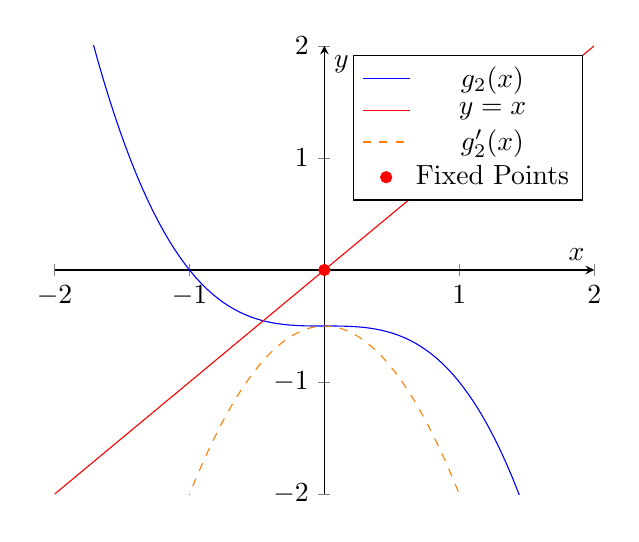
\begin{tikzpicture}
            \begin{axis}[
                    axis lines = middle,
                    xlabel = \( x \),
                    ylabel = \( y \),
                    xmin = -2, xmax = 2,
                    ymin = -2, ymax = 2,
                ]
                \addplot[domain=-2:2, samples=100, color=blue]{-(x^3 + 1) / 2};
                \addplot[domain=-2:2, samples=100, color=red]{x};
                \addplot[domain=-2:2, samples=100, color=orange, dashed]{-(3 * x^2 + 1) / 2};

                \addplot[only marks, mark=*, color=red] coordinates {(0, 0)};

                \addlegendentry{\( g_2(x) \)}
                \addlegendentry{\( y = x \)}
                \addlegendentry{\( g_2'(x) \)}
                \addlegendentry{Fixed Points}
            \end{axis}
        \end{tikzpicture}
        \caption{Graph of \( g_2(x) = -\frac{1}{2} (x^3 + 1) \). The fixed point of \( g_2 \) is the point on \( g_2 \) intersecting the line \( y = x \): \( x = 0 \)}
    \end{figure}

    The basin of attraction of \( g_2 \) for \( x^\ast = 0 \) is \( -1 < x < 1 \).
\end{example}

\subsubsection{Summarization of Theorems}

\begin{remark}[Fixed Point Theorem]
    Let \( g(x) \in C[a, b] \) be such that \( g(x) \in [a, b] \) for all \( x \in [a, b] \). Suppose in addition, \( g \) is differentiable on \( (a, b) \) and \( |g'(x) \leq k < 1 \) for some constant \( k \) and all \( x \in (a, b) \).

        {~~~}

    Then, for any\( x_0 \in [a, b] \) the fixed point iteration \[
        x_{i+1} = g(x_i) \qquad \text{for } i = 0, 1, 2, \dots
    \] converges to the fixed point \( x^\ast \in [a, b] \).
\end{remark}

\begin{example}[Exercise]
    Apply the fixed point theorem to the function \[
        f(x) = x -0.2 \sin(x) - 0.5
    \] with fixed point problem \[
        g(x) = 0.2 \sin(x) + 0.5
    \] and interval \( [-1, 1] \).
\end{example}

\section{Newton's Method}

Back to the root finding problem, we pick \( x_0 \). Then, we approximate \( f(x) \) near \( x_0 \) by a line that goes through \( (x_0), f(x_0) \) with slope \( f'(x_0) \), \[
    \ell: y - f(x_i) = f'(x_i) (x - x_0)
\]

\begin{figure}[H]
    \centering
    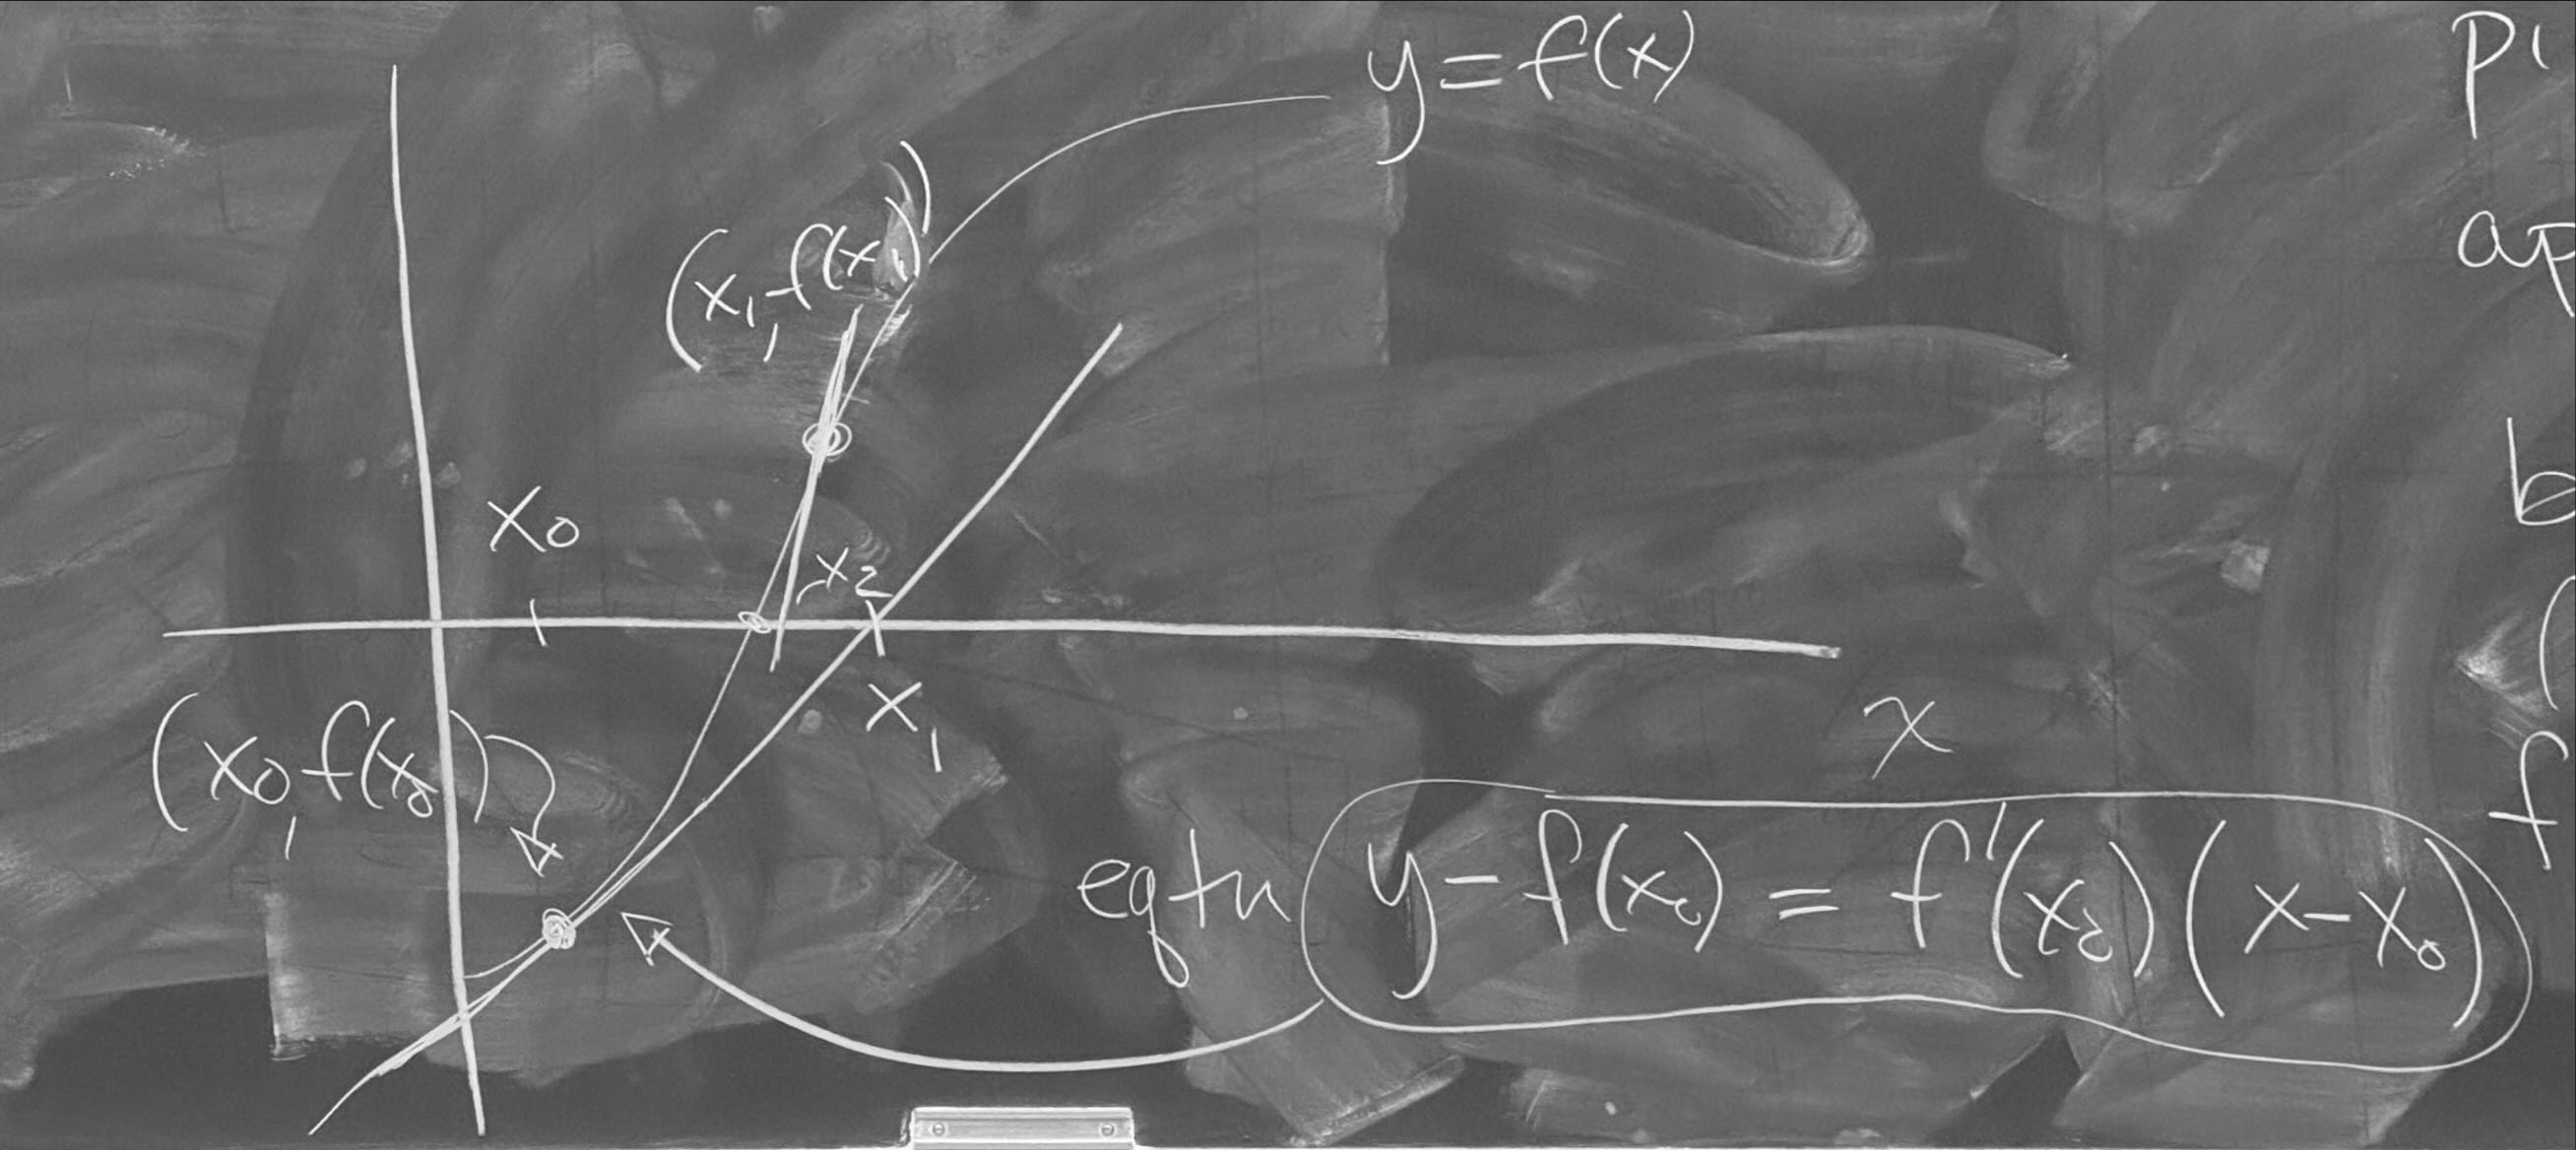
\includegraphics[width=0.67\linewidth]{figures/newtons_method.jpeg}
\end{figure}

Set \( y = 0 \), solve for \( x \) to get the root of the line, \[
    x = x_0 - \frac{f(x_0)}{f'(x_0)}
\]
This gives us a new approximation \( x_1 \) of the root. We repeat this process to get \[
    x_{i+1} = x_i - \frac{f(x_i)}{f'(x_i)} \qquad \text{for } i = 0, 1, 2, \dots
\] and this process is known as \term{Newton's method}.\index{Newton's Method}\index{Newton-Raphson Method}

\begin{definition}[Newton's Method]
    Given \( x_0 \) and \( f(x) \), the sequence of approximations to the root of \( f(x) \) is defined by \[
        x_{i+1} = x_i - \frac{f(x_i)}{f'(x_i)}
    \] for \( i = 0, 1, 2, \dots \)
\end{definition}

\begin{example}
    Suppose we want to find the roots of the function \[
        f(x) = x - 0.2\sin(x) - 0.5
    \] with \( x_0 = 0 \) until \( |x_{i+1} - x_i| \leq 5 \times 10^{-7} \).

        {~~~}

    Recall that
    \begin{itemize}
        \item Using bisection with \( [L_0, R_0] = [0, 1] \), we need 21 iterations
        \item Using fixed point iteration with \( g(x) = 0.2 \sin(x) + 0.5 \), we need 9 iterations
    \end{itemize} and we now examine the Newton's method.

    We have iterations \[
        x_{i+1}
        = x_i - \frac{f(x_i)}{f'(x_i)}
        = \frac{x_i - 0.2\sin(x_i) - 0.5}{1 - 0.2\cos(x_i)}
    \]

    \begin{table}[H]
        \centering
        \begin{tabular}{c|c|c}
            \( i \)
             & \( x_i \)
             & \( \delta x_i = | x_{i+1} - x_i | \)
            \\ \hline \hline
            \(0\)
             & \(0\)
             &                                      \\
            \(1\)
             & \(0.625\)
             & \(6.3\times10^{-1}\)                 \\
            \(2\)
             & \(0.6154745\ldots\)
             & \(9.5\times10^{-3}\)                 \\
            \(3\)
             & \(0.6154682\ldots\)
             & \(6.3\times10^{-6}\)                 \\
            \(4\)
             & \(0.6154682\ldots\)
             & \(2.8\times10^{-12}\)                \\
        \end{tabular}
        \caption{Newton's method for \( f(x) = x - 0.2 \sin(x) - 0.5 \)}
    \end{table}

    \begin{note}
        We met criteria in \( 4 \) steps, and we observe quadratic convergence.

        \begin{itemize}
            \item In bisection methods, we only use the sign of \( f(x) \), which is only 1 bit of information.
            \item In Newton's methods, we use the slope of \( f(x) \) at \( x_i \), which provides more information about the function.
        \end{itemize}
    \end{note}
\end{example}

\section{Secant Method}

Finding the derivative may be complicated and error-prone, and we can use the secant method instead. Instead, we could use two initial approximations \( x_0, x_1 \) and the secant line that goes through \[
    (x_0, f(x_0)), (x_1, f(x_1))
\] to approximate the root. The secant line is given by \[
    y - f(x_1) = \frac{f(x_1) - f(x_0)}{x_1 - x_0} (x - x_1)
\] We are interested in the \(x\)-intercept of the secant line, so we can set \( y = 0 \) and re-arrange to get \[
    x = x_1 - \frac{f(x_1)(x_1 - x_0)}{f(x_1) - f(x_0)}
\] This gives us a new approximation \( x_2 \) of the root. We repeat this process to get \[
    x_{i+1} = x_i - \frac{f(x_i)(x_i - x_{i-1})}{f(x_i) - f(x_{i-1})} \qquad \text{for } i = 1, 2, \dots
\] This is known as the \term{secant method}.\index{Secant Method}

\begin{definition}[Secant Method]
    Given \( x_0, x_1 \) and \( f(x) \), the sequence of approximations to the root of \( f(x) \) is defined by \[
        x_{i+1} = x_i - \frac{f(x_i)(x_i - x_{i-1})}{f(x_i) - f(x_{i-1})}
    \] for \( i = 1, 2, \dots \)
\end{definition}

\begin{remark}[Comparison with Newton's Method]
    In Newton's method, we need to compute \( f(x_i) \) and \( f'(x_i) \) in each iteration, where as in secant method, we only need to compute \( f(x_i) \) (\( f(x_{i-1}) \) is already computed in the previous iteration). This is useful when \( f'(x) \) is difficult to compute.

        {~~~}

    In general, the secant method will require less work per iteration than Newton's method, but it will converge slower.
\end{remark}

\begin{example}
    Find the roots of \[
        f(x) = x - 0.2 \sin(x) - 0.5
    \] with \( x_0 = 0, x_1 = 1 \) until \( |x_{i+1} - x_i| \leq 5 \times 10^{-7} \).

    \begin{table}[H]
        \centering
        \begin{tabular}{c|c|c}
            \( i \)
             & \( x_i \)
             & \( \Delta x_i = | x_{i+1} - x_i | \)
            \\ \hline \hline
            0
             & \( 0 \)
             &
            \\
            1
             & \( 1 \)
             &
            \\
            2
             & \( 0.6011741\ldots \)
             & \( 4.0 \times 10^{-1} \)
            \\
            3
             &
            \( 0.6150404\ldots \)
             & \( 1.4 \times 10^{-2} \)
            \\
            4
             & \( 0.6154686\ldots \)
             & \( 4.3 \times 10^{-4} \)
            \\
            5
             & \( 0.6154682\ldots \)
             & \( 4.2 \times 10^{-7} \)
        \end{tabular}
        \caption{Secant method for \( f(x) = x - 0.2 \sin(x) - 0.5 \)}
    \end{table}
    We meet the stopping criteria in 4 steps.

    Recall that in Newton method, we also converged in 4 steps, but the error was much smaller.
\end{example}

\begin{remark}
    Both Newton's method and secant method \textbf{can} converge quickly. However, they \textbf{do not guarantee convergence}.
\end{remark}

\section{Rate of Convergence}

\subsection{Rate of Convergence for Different Methods}

Suppose we generate a sequence \( x_0, x_1, x_2, \dots \) that converges to \( x^\ast \).

Let \[
    e_i = | x_i - x^\ast | \qquad \text{for } i = 0, 1, 2, \dots
\] be the absolute error in \( x_i \)\footnote{Sometimes, \( e_i \) is the \textit{bound} on the error, for example, in the bisection method.}.

The \term{rate of convergence} \( r \) of the sequence is the largest \( r \) such that \[
    \lim_{\substack{x \to x\ast}} \frac{e_{i+1}}{(e_i)^r} = C \neq 0 \text{ (constant)}
\]

\begin{itemize}
    \item In bisection method, \[
              e_{i+1} = \frac{1}{2} e_i
          \] so \[
              \lim_{\substack{x \to x\ast}} \frac{e_{i+1}}{(e_i)^1} = \frac{1}{2}
          \] and \( r = 1 \)

          This suggests \textbf{linear convergence}.

          \begin{note}
              If \( r > 1 \), then the convergence is \term{superlinear}.
          \end{note}

    \item In Newton's method, conctruct a Tayler series approximation of \( f(x) \) near \( x^\ast \)

          We know that \begin{align*}
              0 & = f(x^\ast)
              \\
                & = f(x_i + (x^\ast) - x_i)
              \\
                & = f(x_i) + f'(x_i) (x^\ast - x_i) + \frac{1}{2} f''(\Theta) (x^\ast - x_i)^2
          \end{align*}
          for some \( \Theta \) between \( x_i \) and \( x^\ast \).

          Assuming \( f'(x_i) \) exists and is non-zero, we can divide both sides by \( f'(x_i) \) to get \begin{align*}
              0
               & = \frac{f(x_i)}{f'(x_i)} + (x^\ast - x_i) + \frac{1}{2} \frac{f''(\Theta)}{f'(x_i)} (x^\ast - x_i)^2
              \\
              x^\ast - \left( x_i - \frac{f(x_i)}{f'(x_i)} \right)
               & = -\frac{1}{2} \frac{f''(\Theta)}{f'(x_i)} (x^\ast - x_i)^2
              \\
              x^\ast - x_{i+1}
               & = - \frac{f''(\Theta)}{2f'(x_i)} (x^\ast - x_i)^2
              \\
              e_{i+1}
               & = \left| \frac{f''(\Theta)}{2f'(x_i)} \right| {e_i}^2
          \end{align*}
          If the method converges, \[
              \lim_{\substack{x \to x\ast}} \frac{e_{i+1}}{(e_i)^2} = \left| \frac{f''(\Theta)}{2f'(x_i)} \right| \neq 0
          \] and the rate of convergence is \( 2 \), which is \term{superlinear}.

          \begin{remark}
              If \( f'(x_i) = 0 \), then we have multiple roots, and converges to \( r = 1 \).
          \end{remark}

    \item In secant method, we can show \[
              \lim_{\substack{x \to x\ast}} \frac{e_{i+1}}{e_i e_{i-1}} = C \neq 0
          \] and then show \[
              \lim_{\substack{x \to x\ast}} \frac{e_{i+1}}{(e_i)^r} = C \neq 0
          \] for \[
              r = \frac{1 + \sqrt{5}}{2} \approx 1.618
          \] which is the \term{golden ratio}.
\end{itemize}

\subsection{Interpretation of Rate of Convergence}

TODO: See plot.